\documentclass[a4paper]{scrartcl}
\usepackage[english]{babel}
\usepackage[top=2cm,bottom=3cm,left=2.5cm,right=2.5cm]{geometry}
\usepackage[colorlinks=true, allcolors=black]{hyperref}
\usepackage{wrapfig} %문단 내 이미지 삽입
\usepackage{graphicx} %색상
\usepackage{overpic}
\usepackage[normalem]{ulem}%취소선
\usepackage{array} %표
\usepackage{mdframed, tcolorbox} %글상자
	\newcommand{\asw}[2]{
		\begin{flushright}
			{\color{black}#1 \quad $\blacktriangleleft$\quad #2}
		\end{flushright}
	}
\usepackage[yyyymmdd]{datetime}
\renewcommand{\dateseparator}{-}
\usepackage{amsmath, amsfonts, amssymb, bm} %수식
	\DeclareMathOperator{\arccsc}{arccsc}
	\DeclareMathOperator{\arcsec}{arcsec}
	\DeclareMathOperator{\arccot}{arccot}
	\DeclareMathOperator{\csch}{csch}
	\DeclareMathOperator{\sech}{sech}
	\DeclareMathOperator{\arcsinh}{arcsinh}
	\DeclareMathOperator{\arccosh}{arccosh}
	\DeclareMathOperator{\arctanh}{arctanh}
	\DeclareMathOperator{\arccsch}{arccsch}
	\DeclareMathOperator{\arcsech}{arcsech}
	\DeclareMathOperator{\arccoth}{arccoth}
	
	\DeclareMathOperator{\meter}{m}
	\DeclareMathOperator{\cm}{cm}
	\DeclareMathOperator{\mm}{mm}
	\DeclareMathOperator{\mum}{\mu m}
	\DeclareMathOperator{\newton}{N}
	\DeclareMathOperator{\kn}{kN}
	\DeclareMathOperator{\kgf}{kgf}
	\DeclareMathOperator{\pa}{Pa}
	\DeclareMathOperator{\kpa}{kPa}
	\DeclareMathOperator{\mpa}{MPa}
	\DeclareMathOperator{\gpa}{GPa}
	\DeclareMathOperator{\knpm}{kN/m}
	\DeclareMathOperator{\kph}{km/h}
	\DeclareMathOperator{\mps}{m/s}
	\DeclareMathOperator{\tkph}{kph}
	\DeclareMathOperator{\tmps}{mps}
	\DeclareMathOperator{\mpss}{m/s^2}
	\DeclareMathOperator{\dgr}{\!^\circ}
	\DeclareMathOperator{\cel}{\!^\circ C}
	\DeclareMathOperator{\kg}{kg}
	\DeclareMathOperator{\kgpcm}{kg/m^3}
	\DeclareMathOperator{\knm}{kN\cdot m}
	\DeclareMathOperator{\nm}{N\cdot m}
	\DeclareMathOperator{\watt}{W}
	\DeclareMathOperator{\kw}{kW}
	\DeclareMathOperator{\kwh}{kWh}
	\DeclareMathOperator{\mmhg}{mmHg}
	\DeclareMathOperator{\snd}{s}
	\DeclareMathOperator{\hz}{Hz}
\usepackage{polynom} %나눗셈 필산
\usepackage{cancel} %수식 약분선
\usepackage{titlesec} %섹션 이름 변경
	\titlespacing*{\section}{3mm}{0mm}{1mm}
	\titleformat{\section}{\bfseries\large}{}{0ex}{}
\usepackage{kotex} %한글

\title{\vspace{100pt}\Huge{HW4}}
\author{
	2025-1 고체역학(박성훈 교수님)\\[10pt]
	Problem 3.67, 3.68, 3.71, 3.74, 3.92, 3.95, 3.98, 3.116\\[110pt]
	}
\date{\today}

\begin{document}
	
\renewcommand*{\titlepagestyle}{empty}
\maketitle
\setlength{\parindent}{3mm}

\vspace{60pt}

\begin{center}
	\includegraphics[width=0.45\textwidth]{SSU symbol KR-EN.jpg}
\end{center}

\newpage
\setcounter{page}{1}

\section{Problem 3.67}
	\begin{mdframed}
		Determine the maximum shearing stress in a solid shaft of 18-mm diameter as it transmits $3.4\kw$ at a frequency of ($a$) $25\,\text{Hz}$, ($b$) $50\,\text{Hz}$.
	\end{mdframed}
	\begin{align*}
		&c = 9\mm,\quad T = \frac{P}{2\pi f},\quad J = \frac{\pi}{2}c^4\\
		&\tau_{\text{max}} = \frac{Tc}{J} = \frac{P}{\pi^2 f c^3}
	\end{align*}
	When ($a$) $f = 25\hz$,
	\begin{align*}
		&\tau_{\text{max}} = \frac{3.4\kw}{\pi^2(25\hz)(9\mm)^3} = \frac{3400}{\pi^2(25)(0.009)^3}\pa = 18.90\mpa\quad\blacktriangleleft\quad(a)
	\end{align*}
	When ($b$) $f = 50\hz$,
	\begin{align*}
		&\tau_{\text{max}} = \frac{3.4\kw}{\pi^2(50\hz)(9\mm)^3} = \frac{3400}{\pi^2(25)(0.009)^3}\pa = 9.45\mpa\quad\blacktriangleleft\quad(b)
	\end{align*}

\vspace{10pt}

\section{Problem 3.68}
	\begin{mdframed}
		While a steel shaft of the cross section shown rotates at 120 rpm, a stroboscopic measurement indicates that the angle of twist is $2\dgr$ in a 4-m length. Using $G = 77.2\gpa$, determine the power being transmitted.
		\begin{center}
			\includegraphics[width = 60mm]{img/P3-68.png}
		\end{center}
	\end{mdframed}
	\begin{align*}
		&f = 120\,\mathrm{rpm} = 2\hz,\quad \phi = 2\dgr = \frac{\pi}{90}\;(\mathrm{rad})\\
		&J = \frac{\pi}{2}\left\{\left(\frac{75}{2}\mm\right)^4 - \left(\frac{30}{2}\mm\right)^4\right\} = 3.026789531\times10^{-6}\meter^4\\
		&T = \frac{G\phi J}{L},\quad T = \frac{P}{2\pi f}\\
		&\frac{P}{2\pi f} = \frac{G\phi J}{L}\\
		&P = \frac{2\pi f G \phi J}{L} = \frac{2\pi(2\hz)(77.2\gpa)\left(\frac{\pi}{90}\right)(3.026789531\times10^{-6}\meter^4)}{4\meter}\\
		&\quad = \frac{2\pi(2)(77.2\times10^9)\left(\frac{\pi}{90}\right)(3.026789531\times10^{-6})}{4}\watt = 25.6\kw\quad\blacktriangleleft
	\end{align*}

\newpage

\section{Problem 3.71}
	\begin{mdframed}
		The hollow steel shaft shown ($G = 77.2\gpa$, $\tau_{\text{all}} = 50\mpa$) rotates at 240 rpm. Determine ($a$) the maximum power that can be transmitted, ($b$) the corresponding angle of twist of the shaft.
		\begin{center}
			\includegraphics[width = 60mm]{img/P3-71.png}
		\end{center}
	\end{mdframed}
	\begin{align*}
		&f = 240\,\mathrm{rpm} = 4\hz\\
		&J = \frac{\pi}{2}\left\{\left(\frac{60}{2}\mm\right)^4 - \left(\frac{25}{2}\mm\right)^4\right\} = 1.233995505\times10^{-6}\meter^4\\
		&T_{\text{max}} = \frac{\tau_{\text{all}} J}{c},\quad P_{\text{max}} = 2\pi fT_{\text{max}}\\
		&P_{\text{max}} = \frac{2\pi f\tau_{\text{all}} J}{c} = \frac{2\pi(4\hz)(50\mpa)(1.233995505\times10^{-6}\meter^4)}{30\mm}\\
		&\qquad = \frac{2\pi(4)(50\times10^{6})(1.233995505\times10^{-6})}{0.03}\watt = 51.7\kw\quad\blacktriangleleft\quad(a)\\
		&\phi_{\text{max}} = \frac{\gamma_{\text{all}} L}{c} = \frac{\tau_{\text{all}} L}{Gc} = \frac{(50\mpa)(5\meter)}{(77.2\gpa)(30\mm)} = \frac{(50\times10^6)(5)}{(77.2\times10^9)(0.03)} = \frac{125}{1158} = 6.18\dgr\quad\blacktriangleleft\quad(b)
	\end{align*}

\newpage

\section{Problem 3.74}

	\begin{mdframed}
	\begin{tabular}{m{60mm}m{85mm}}
		\includegraphics[width = 60mm]{img/P3-74.png}
		&
		Three shafts and four gears are used to form a gear train that will transmit power from the motor at $A$ to a machine tool at $F$. (Bearings for the shafts are omitted in the sketch.) The diameter of each shaft is as follows: $d_{AB} = 16\mm$, $d_{CD} = 20\mm$, $d_{EF} = 28\mm$. Knowing that the frequency of the motor is $24\hz$ and that the allowable shearing stress for each shaft is $75\mpa$, determine the maximum power that can be transmitted.
	\end{tabular}
	\end{mdframed}
	\begin{align*}
		&T_{\text{max}} = \cfrac{\tau_{\text{all}} J}{c},\quad P_{\text{max}} = 2\pi f T_{\text{max}} = \cfrac{2\pi f\tau_{\text{all}} J}{c}\\
		&f_{AB} = 24\hz,\quad f_{CD} = \cfrac{60\mm}{150\mm}\,f_{AB} = 9.6\hz,\quad f_{EF} = \cfrac{60\mm}{150\mm}\,f_{CD} = 3.84\hz\\
		&J_{AB} = \frac{\pi}{2}\left(\frac{d_{AB}}{2}\right)^4 = \frac{\pi}{2}\left(8\mm\right)^4 = 2.048\pi\times10^{-9}\meter^4\\
		&P_{\text{max},AB} = \frac{2\pi(24\hz)(75\mpa)(2.048\pi\times10^{-9}\meter^4)}{8\mm} = \frac{2\pi(24)(75\times10^{6})(2.048\pi\times10^{-9})}{0.008}\watt\\
		&\phantom{P_{\text{max},AB}} = 9.10\kw\\[10pt]
		&J_{CD} = \frac{\pi}{2}\left(\frac{d_{CD}}{2}\right)^4 = \frac{\pi}{2}\left(10\mm\right)^4 = 5\pi\times10^{-9}\meter^4\\
		&P_{\text{max},CD} = \frac{2\pi(9.6\hz)(75\mpa)(5\pi\times10^{-9}\meter^4)}{10\mm} = \frac{2\pi(9.6)(75\times10^{6})(5\pi\times10^{-9})}{0.01}\watt\\
		&\phantom{P_{\text{max},CD}} = 7.11\kw\\[10pt]
		&J_{EF} = \frac{\pi}{2}\left(\frac{d_{EF}}{2}\right)^4 = \frac{\pi}{2}\left(14\mm\right)^4 = 1.9208\pi\times10^{-9}\meter^4\\
		&P_{\text{max},EF} = \frac{2\pi(3.84\hz)(75\mpa)(1.9208\pi\times10^{-9}\meter^4)}{14\mm} = \frac{2\pi(3.84)(75\times10^{6})(1.9208\pi\times10^{-9})}{0.014}\watt\\
		&\phantom{P_{\text{max},CD}} = 7.80\kw\\[10pt]
		&9.10\kw > 7.80\kw > 7.11\kw \quad\Rightarrow\quad P_{\text{max}} = 7.11\kw\quad\blacktriangleleft
	\end{align*}
	
\newpage

\section{Problem 3.92}
	\begin{mdframed}
		The solid circular shaft shown is made of a steel that is assumed to be elastoplastic with $\tau_{Y} = 145\mpa$. Determine the magnitude $T$ of the applied torques when the plastic zone is ($a$) $16\mm$ deep, ($b$) $24\mm$ deep.
		\begin{center}
			\includegraphics[width = 60mm]{img/P3-92.png}
		\end{center}
	\end{mdframed}
	\begin{align*}
		&J = \frac{\pi}{2}c^4 = \frac{\pi}{2}(32\mm)^4 = 5.24288\pi\times10^{-7}\meter^4\\
		&T_Y = \frac{\tau_Y J}{c} = \frac{(145\mpa)(5.24288\pi\times10^{-7}\meter^4)}{32\mm} = \frac{(145\times10^6)(5.24288\pi\times10^{-7})}{0.032}\nm\\
		&\quad = 7.463418835\knm
	\end{align*}
	When $\rho_Y = 16\mm$,
	\begin{align*}
		&\frac{\rho_Y}{c} = \frac{16\mm}{32\mm} = \frac{1}{2}\\
		&T = \frac{4}{3}T_Y\left\{1-\frac{1}{4}\left(\frac{\rho_Y}{c}\right)^3\right\} = \frac{4}{3}T_Y\left\{1-\frac{1}{4}\left(\frac{1}{2}\right)^3\right\} = \frac{31}{24}T_Y = \frac{31}{24}(7.463418835\knm)\\
		&\quad = 9.64\knm\quad\blacktriangleleft\quad(a)
	\end{align*}
	When $\rho_Y = 32\mm - 24\mm = 8\mm$,
	\begin{align*}
		&\frac{\rho_Y}{c} = \frac{8\mm}{32\mm} = \frac{1}{4}\\
		&T = \frac{4}{3}T_Y\left\{1-\frac{1}{4}\left(\frac{\rho_Y}{c}\right)^3\right\} = \frac{4}{3}T_Y\left\{1-\frac{1}{4}\left(\frac{1}{4}\right)^3\right\} = \frac{85}{64}T_Y = \frac{85}{64}(7.463418835\knm)\\
		&\quad = 9.91\knm\quad\blacktriangleleft\quad(b)
	\end{align*}

\newpage
	
\section{Problem 3.95}
	\begin{mdframed}
		The solid shaft shown is made of a mild steel that is assumed to be elastoplastic with $G = 77.2\gpa$ and $\tau_Y = 145\mpa$. Determine the maximum shearing stress and the radius of the elastic core caused by the application of a torque of magnitude ($a$) $T$ = 600 N-m, ($b$) $T$ = 1000 N-m.
		\begin{center}
			\includegraphics[width = 50mm]{img/P3-95.png}
		\end{center}
	\end{mdframed}
	\begin{align*}
		&c = \frac{30\mm}{2} = 15\mm\\
		&J = \frac{\pi}{2}c^4 = \frac{\pi}{2}(15\mm)^4 = 2.53125\pi\times10^{-8}\meter^4\\
		&T_Y = \frac{\tau_Y J}{c} = \frac{(145\mpa)(2.53125\pi\times10^{-8}\meter^4)}{15\mm} = \frac{(145\times10^6)(2.53125\pi\times10^{-8})}{0.015}\nm\\
		&\quad = 768.7084524\nm
	\end{align*}
	When ($a$) $T = 600\nm < T_Y$,
	\begin{align*}
		&\tau_{\text{max}} = \frac{Tc}{J} = \frac{(600\nm)(15\mm)}{2.53125\pi\times10^{-8}\meter^4} = \frac{(600)(0.015)}{2.53125\pi\times10^{-8}}\pa = 113.2\mpa\\
		&\rho_Y = c = 15\mm
	\end{align*}
	\asw{$113.2\mpa\,;\,15.00\mm$}{($a$)}
	When ($b$) $T = 1000\nm > T_Y$,
	\begin{align*}
		&\tau_{\text{max}} = \tau_Y = 145\mpa\\
		&T = \frac{4}{3}T_Y\left\{1-\frac{1}{4}\left(\frac{\rho_Y}{c}\right)^3\right\}\\
		&\rho_Y = c\sqrt[3]{4 - \frac{3T}{T_Y}} = (15\mm)\sqrt[3]{4 - \frac{3(1000\nm)}{768.7084524\nm}} = 6.90\mm
	\end{align*}
	\asw{$145.0\mpa\,;\,6.90\mm$}{($b$)}

\newpage

\section{Problem 3.98}
	\begin{mdframed}
		The solid shaft shown is made of a mild steel that is assumed to be elastoplastic with $G = 77.2\gpa$ and $\tau_Y = 145\mpa$. Determine the angle of twist caused by the application of a torque of magnitude ($a$) $T$ = 600 N-m, (b) $T$ = 1000 N-m.
		\begin{center}
			\includegraphics[width = 50mm]{img/P3-98.png}
		\end{center}
	\end{mdframed}
	From the solution of Prob.3.95,
	\begin{align*}
		&J = 2.53125\pi\times10^{-8}\meter^4\\
		&T_Y = 768.7084524\nm
	\end{align*}
	When ($a$) $T = 600\nm < T_Y$,
	\begin{align*}
		&\phi = \frac{TL}{GJ} = \frac{(600\nm)(1.2\meter)}{(77.2\gpa)(2.53125\pi\times10^{-8}\meter^4)} = \frac{(600)(1.2)}{(77.2\times10^9)(2.53125\pi\times10^{-8})} = 6.72\dgr\\
		&\hspace{138mm}\blacktriangle\quad(a)
	\end{align*}
	When ($b$) $T = 1000\nm > T_Y$,
	\begin{align*}
		&\phi_Y = \frac{\gamma_Y L}{c} = \frac{\tau_Y L}{Gc} = \frac{(145\mpa)(1.2\meter)}{(77.2\gpa)(15\mm)} = \frac{(145\times10^6)(1.2)}{(77.2\times10^9)(0.015)} = \frac{29}{193}\\
		&T = \frac{4}{3}T_Y\left\{1-\frac{1}{4}\left(\frac{\phi_Y}{\phi}\right)^3\right\}\\
		&\phi = \phi_Y\left(4 - \frac{3T}{T_Y}\right)^{-\frac{1}{3}} = \frac{29}{193}\left(4-\frac{3(1000\nm)}{768.7084524\nm}\right)^{-\frac{1}{3}} = 18.71\dgr\quad\blacktriangleleft\quad(b)
	\end{align*}
	
\newpage
	
\section{Problem 3.116}
	\begin{mdframed}
		The solid shaft shown is made of a steel that is assumed to be elastoplastic with $\tau_Y = 145\mpa$ and $G = 77.2\gpa$. The torque is increased in magnitude until the shaft has been twisted through $6\dgr$; the torque is then removed. Determine ($a$) the magnitude and location of the maximum residual shearing stress, ($b$) the permanent angle of twist.
		\begin{center}
			\includegraphics[width = 55mm]{img/P3-116.png}
		\end{center}
	\end{mdframed}
	\begin{align*}
		&J = \frac{\pi}{2}c^4 = \frac{\pi}{2}(16\mm)^4 = 3.2768\pi\times10^{-8}\meter^4\\
		&T_Y = \frac{\tau_Y J}{c} = \frac{(145\mpa)(3.2768\pi\times10^{-8}\meter^4)}{16\mm} = \frac{(145\times10^6)(3.2768\pi\times10^{-8})}{0.016}\nm\\
		&\quad = 932.9273544 \nm\\
		&\phi_Y = \frac{\tau_Y L}{Gc} = \frac{(145\mpa)(0.6\meter)}{(77.2\gpa)(16\mm)} = \frac{(145\times10^6)(0.6)}{(77.2\times10^9)(0.016)} = \frac{435}{6176} = 4.035567372\dgr\\
		&R = \frac{\rho_Y}{c} = \frac{\phi_Y}{\phi} = \frac{4.035567372\dgr}{6\dgr} = 0.672594562 
	\end{align*}
	\includegraphics{img/Q3-116-1.png}
	\begin{align*}
		\text{loading :}\quad &T = \frac{4}{3}T_Y\left(1-\frac{1}{4}R^3\right) = \frac{4}{3}(932.9273544\nm)\left\{1-\frac{1}{4}(0.672594562)^3\right\}\\
		&\quad = 1149.282337\nm\\
		\text{un-loading :}\quad &T' = \frac{\tau'_{\text{max}}J}{c}\\
		&T = T',\quad T = \frac{\tau'_{\text{max}}J}{c}\\
		&\tau'_{\text{max}} = \frac{Tc}{J} = \frac{(1149.282337\nm)(16\mm)}{3.2768\pi\times10^{-8}\meter^4} = \frac{(1149.282337)(0.016)}{3.2768\pi\times10^{-8}}\pa\\
		&\quad = 178.6269189\mpa\\
		&\tau_{\text{res}}(\rho) = |\tau(\rho) - \tau'(\rho)|\\
		&\tau_{\text{res}}(\rho_Y) = |\tau(\rho_Y) - \tau'(\rho_Y)| = |\tau_Y - R\tau'_{\text{max}}| \\
		&\qquad\quad = |145\mpa - (0.672594562)(178.6269189\mpa)| = 24.9\mpa
	\end{align*}
	\begin{align*}
		&\tau_{\text{res}}(c) = |\tau(c) - \tau'(c)| = |\tau_Y - \tau'_{c}| = |145\mpa - 178.6269189\mpa|\\
		&\qquad\quad = 33.6\mpa\\
		&\left.\begin{array}{r}
			\tau_{\text{res}}(\rho_Y) = 24.9\mpa\\
			\tau_{\text{res}}(c) = 33.6\mpa
		\end{array}\right\}\quad\Rightarrow\quad \tau_{\text{res,max}} = 33.6\mpa
	\end{align*}
	\asw{$33.6\mpa$\quad at\quad $\rho = 16.00\mm$}{($a$)}
	\hspace{30mm}\includegraphics{img/Q3-116-2.png}
	\begin{align*}
		&\phi_p = \phi - \phi' = \phi - T\cdot\frac{\phi_Y}{T_Y} = 6\dgr - \frac{1149.282337\nm}{932.9273544\nm}(4.035567372\dgr) = 1.028\dgr\quad\blacktriangleleft\quad(b)
	\end{align*}

\end{document}